% % % % % % % % % % % % % % % % 
\section{Work Plan}\label{chapterlabel4sec2}

The PhD contributions so far demonstrate the value for an MRI simulation framework capable of producing realistic MRI datasets of advanced sequences in an accurate and rapid manner.
Future work will therefore include:

\begin{enumerate}
    \item \textit{Write an MRI simulators review paper.}
    So far, we have investigated the current state-of-the art in MRI simulation systems and experimented with 2 of the most popular and active MRI simulators today.
    It is our plan for the future to focus on fleshing out the literature review of this thesis into a review paper.
    We estimate that this will take 3 months to complete (see first entry in Figure~\ref{fig:ganttChart}). 

	\item \textit{Continue with motion-corrupted MRF experiments.}
	So far, we have investigated how in-plane motion corrupts the MRF quantitative maps.
	In the future we will investigate through-plane motion and a combination of both in-plane and through-plane motion for the original MRF implementation by Ma et al. \cite{Ma2013}.
	We estimate 3 months for this to be completed (see second entry in Figure~\ref{fig:ganttChart}).
	
	\item \textit{Develop an open-source MRI simulator that will allow for the simulation of advanced MRI sequences.}
	So far, we have implemented a proof-of-concept simulation framework for a Magnetic Resonance Fingerprinting experiment in an open-source simulator called JEMRIS \cite{Stocker2010}.
	However, in order to mimic a continuous distribution of spins throughout an object voxel, a high number of isochromats is required to generate a smooth image intensity \cite{Shkarin1997}.
	Moreover, newer MRF implementations rely on an imaging sequence called fast imaging with steady state precession (FISP, see Appendix \ref{MRIFISP}) which requires an even denser collection of spins to be accurate.
	With the current JEMRIS implementation, such experiments would require an unfeasibly long time to simulate.
	For this reason it is our plan for future work to develop an open-source MRI simulator based on GPU parallelisation and the newest programming standards offered by CUDA 9.x.
	The general framework for this simulator is presented in the next section.
	We estimate 6 months for this to be completed (see third entry in Figure~\ref{fig:ganttChart}). 
	\item \textit{Validate the implementation.}
	So far, the simulation system has not been validated.
	This is because the real MRF datasets that we have are for the MRF-FISP implementation.
	For this reason, we aim to demonstrate the applicability of our new simulator by validating it against real MRF-FISP datasets.
	As software bugs could appear during this process, we estimate 3 months for this to be completed (see fourth entry in Figure~\ref{fig:ganttChart}).
	
	\item \textit{Simulate the impact of motion on the MRF-FISP sequence.}
	After validation, we will be in a great place to investigate the impact of motion on the MRF-FISP sequence.
	For this, we aim to look at in-plane, through-plane and a combination of both in-plane and through-plane motion for the newly developed simulation system.
	We estimate 3 months for this to be completed (see fifth entry in Figure~\ref{fig:ganttChart}).
	
\end{enumerate}

\begin{figure}[ht]
    \centering
    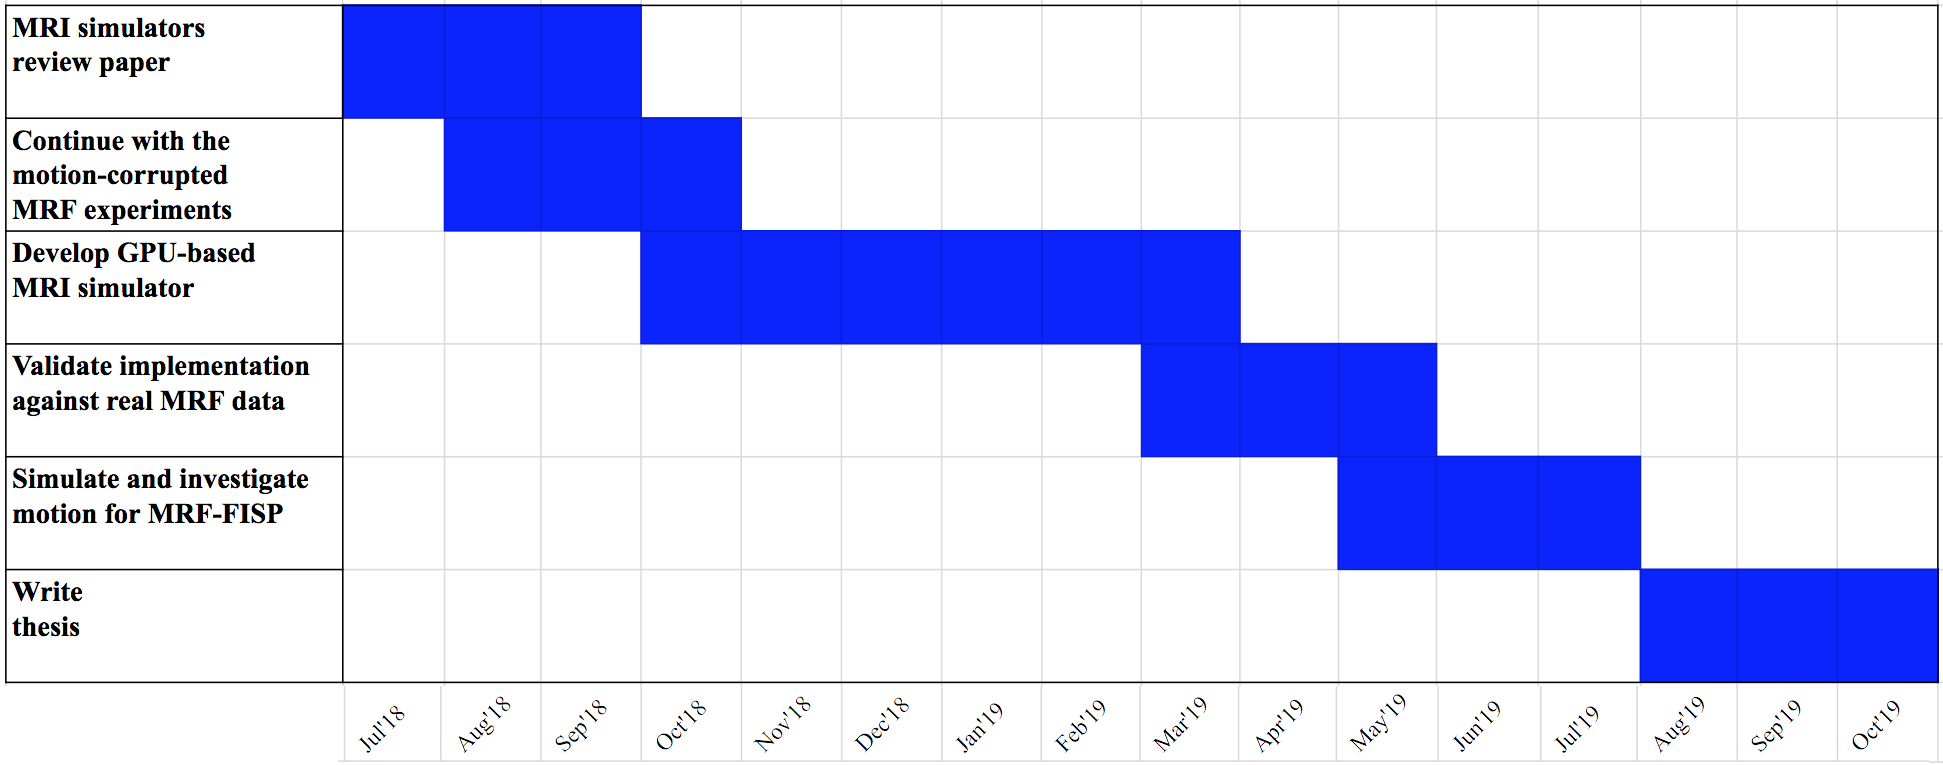
\includegraphics[width=1\textwidth, keepaspectratio]{images/mri/ganttChart}
    \caption{Gantt chart demonstrating how I will spend the remaining time in my PhD}
    \label{fig:ganttChart}
\end{figure}
